\documentclass{article}

\usepackage{booktabs}
\usepackage{multirow}
\usepackage{amsmath}
\usepackage{hyperref}
\usepackage{overpic}
\usepackage{amssymb}
\usepackage{graphicx}
\usepackage{tikz}
\usetikzlibrary{positioning,arrows.meta,calc}

\usepackage[accepted]{dlaiml2026}

\dlaititlerunning{Permutation Alignment and REPAIR for Model Merging in Low-Resource Regimes}

\begin{document}

\twocolumn[
\dlaititle{Permutation Alignment and REPAIR Close the Merging Gap\\in Low-Resource Regimes}

\begin{center}\today\end{center}

\begin{dlaiauthorlist}
\dlaiauthor{Marco Linardi}{}
\end{dlaiauthorlist}

\dlaicorrespondingauthor{Marco Linardi}{linardi.2003980@studenti.uniroma1.it}

\vskip 0.3in
]

\printAffiliationsAndNotice{}

\begin{abstract}
%
Na\"ive weight averaging of independently trained networks succeeds in the linear-mode-connected (LMC) basin of \citet{frankle2020lmc} but is known to fail outside it. We characterise an intermediate regime motivated by federated and distributed-learning settings~\citep{mcmahan2017fedavg}: five ResNet-20 networks sharing initialisation, each trained for 30 epochs on a disjoint $10{,}000$-sample slice of CIFAR-10~\citep{krizhevsky2009cifar}. Uniform soup collapses to $12.62\%$ test accuracy (mean individual $75.20\%$); TIES-Merging~\citep{yadav2023ties} reaches $10.98\%$ at the paper-default $\lambda\!=\!1.0$, and pairwise test-loss barriers grow $30$--$50\times$ above the same-init/full-data reference. A two-step pipeline of Activation Matching~\citep{ainsworth2023rebasin} followed by REPAIR~\citep{jordan2023repair} raises the midpoint accuracy to $76.54\%$ on a different-init pair (within $8.0$\,pp of the endpoints) and to $68.20\!\pm\!0.98\%$ across four low-resource pairs (mean gap $6.8$\,pp). Pairwise task-vector cosine fails to predict mergeability ($r\!=\!+0.28$, $p\!\approx\!0.43$, $n\!=\!10$). Code: \url{https://github.com/MarcoLinardi/Deep-Learning-and-Applied-AI-2025-26-exam-project}.
%
\end{abstract}

% ------------------------------------------------------------------------------
\section{Introduction}

Model merging aggregates independently trained networks into one. Whether accuracy is preserved depends on the loss-landscape geometry: in the LMC regime~\citep{frankle2020lmc} two networks lie on a low-loss linear path; outside it, averaging collapses to chance. We study a federated-learning-motivated intermediate regime~\citep{mcmahan2017fedavg}: shared initialisation, data partitioned so each model sees one fifth of CIFAR-10. Contributions: (i)~LMC breaks in this regime (barriers $30$--$50\times$ the full-data reference); (ii)~Activation Matching~\citep{ainsworth2023rebasin} + REPAIR~\citep{jordan2023repair} restores midpoint accuracy to within $6$--$8$\,pp across five pairs; (iii)~pairwise task-vector cosine fails to predict mergeability.

% ------------------------------------------------------------------------------
\section{Related Work}

\textbf{LMC and permutation alignment.} \citet{frankle2020lmc} characterise when two trained networks are connected by a low-loss linear path; we adopt their error-barrier definition. \citet{ainsworth2023rebasin} exploit the channel-permutation symmetry of CNNs ($\theta\!\mapsto\!\Pi(\theta)$ is invariant for any per-layer $\Pi$): their Activation Matching variant aligns $\theta_B$ to $\theta_A$ by Hungarian assignment on channel-wise activation correlations. \citet{jordan2023repair} observe that a residual barrier persists due to BatchNorm feature-scale drift and propose a brief low-LR fine-tune. Further approaches include OTFusion~\citep{singh2020otfusion} and ZipIt!~\citep{stoica2024zipit}.

\textbf{Soups and task arithmetic.} \citet{wortsman2022soup} introduced uniform and greedy soups; \citet{ilharco2023task} extended the framework to task arithmetic; \citet{yadav2023ties} resolve sign interference with trim/elect/disjoint-merge.

% ------------------------------------------------------------------------------
\section{Method}

\textbf{Architecture and baseline.} ResNet-20~\citep{he2016resnet} on CIFAR-10~\citep{krizhevsky2009cifar}: three stages of three BasicBlocks ($16/32/64$ ch, projection shortcuts; $272{,}474$ parameters). Full-data baseline: 50 epochs, SGD (lr $0.1$, Nesterov momentum $0.9$, weight decay $10^{-4}$, cosine schedule, batch $128$, standard augmentation); reaches $90.10\%$ test accuracy.

\textbf{Low-resource setup (E2).} We deterministically partition the 50k train set into $N\!=\!5$ disjoint $10$k slices (\texttt{partition\_seed=11}) and train five ResNet-20 networks for 30 epochs from the same initialisation (\texttt{init\_seed=0}); per-model SGD seeds differ. Mean final test accuracy: $75.20\%$ (range $74.36$--$76.54\%$).

\textbf{Merging baselines.} (i) best single, (ii)~uniform soup $\theta\!=\!\tfrac{1}{N}\sum_i\theta_i$, (iii)~greedy soup~\citep[Alg.\ 1]{wortsman2022soup}, (iv)~TIES with $k\!=\!0.20$, $\lambda\!=\!1.0$ on $\tau_i\!=\!\theta_i\!-\!\theta_{\text{base}}$. For every merged model we reset BatchNorm statistics on $200$ batches of augmented training data before evaluation; without this step every merged accuracy collapses to $\sim\!10\%$ even when LMC holds.

\textbf{Activation Matching.} ResNet-20 admits twelve independent channel permutations: three \emph{stage-output} permutations (sizes $16,32,64$, one per stage, shared by all blocks because the residual+shortcut sum forces a single permutation) and one \emph{block-internal} permutation per BasicBlock between $\mathrm{conv}_1$ and $\mathrm{conv}_2$ (App.~F). We hook activations at the twelve points, build channel-channel correlation matrices on a $512$-sample no-augmentation calibration batch, solve $\max_P \mathrm{tr}(P^{\!\top}\!C)$ with the Hungarian algorithm and iterate ($\leq\!5$ passes; convergence in $2$).

\textbf{REPAIR.} After the aligned merge $\theta_{\text{merge}}\!=\!\tfrac{1}{2}(\theta_A\!+\!\theta_B')$, BN-reset on $200$ batches and SGD for two epochs on the full CIFAR-10 train set (lr $10^{-3}$, momentum $0.9$, weight decay $10^{-4}$, Nesterov, batch $128$). End-to-end pipeline cost: $\approx\!1$ minute of GPU time per merged pair.

% ------------------------------------------------------------------------------
\section{Results}

\textbf{E2: na\"ive merging fails (App.\,C).} Uniform soup reaches $12.62\%$ and TIES-Merging $10.98\%$, both indistinguishable from random ($10.00\%$). Greedy soup degenerates to a single-model soup of $76.60\%$: it starts from the best individual (\#2, $76.54\%$) but no second model improves the running mean, so the procedure halts immediately (App.\,D). Pairwise test-loss barriers are $30$--$50\times$ the full-data reference~\citep{frankle2020lmc}, confirming LMC failure (App.\,A).

\textbf{E3: AM\,+\,REPAIR closes the gap.} We apply the full pipeline to five pairs: (a)~\texttt{E1D\_pair0}, two networks with different initialisations trained on disjoint halves of CIFAR-10 (the classical Git Re-Basin setting), and (b)--(e)~four low-resource E2 pairs. Iterative Activation Matching alone reduces the test-loss barrier from $2.394$ to $1.676$ on (a) and from $2.370$ to $1.316$ on (b); the midpoint accuracy lifts from $15.38\%$ to $44.89\%$ and from $22.35\%$ to $41.37\%$ on average across the E2 pairs (Tab.~\ref{tab:pipeline}, Fig.~\ref{fig:e3pipeline}). Two REPAIR epochs then raise the midpoint accuracy to $\mathbf{76.54\%}$ on (a) -- within $8.0$\,pp of the parents' average -- and to $\mathbf{68.20\!\pm\!0.98\%}$ on the four E2 pairs (mean gap $6.8$\,pp). The pipeline recovers more than $80\%$ of the random-to-endpoint gap on all pairs.

\begin{table}[t]
\caption{Midpoint test accuracy at three stages of the merging pipeline. ``$\Delta\!\to\!\text{end}$'' is the residual gap to the average endpoint accuracy.}
\label{tab:pipeline}
\begin{center}
\begin{small}
\begin{tabular}{lcc}
\toprule
Stage & E1-D pair & E2 pairs ($n{=}4$) \\
\midrule
endpoint accuracy (avg) & $84.57\%$ & $75.00\%$ \\
\midrule
pre-merge midpoint     & $15.38\%$ & $22.35\%$ \\
+ Activation Matching  & $44.89\%$ & $41.37\%$ \\
+ REPAIR ($2$\,ep, $\eta\!=\!10^{-3}$) & $\mathbf{76.54\%}$ & $\mathbf{68.20\!\pm\!0.98\%}$ \\
\midrule
$\Delta\!\to\!\text{end}$ (post-pipeline) & $\phantom{0}8.03$\,pp & $\phantom{0}6.80$\,pp \\
\bottomrule
\end{tabular}
\end{small}
\end{center}
\vspace{-0.35cm}
\end{table}

\begin{figure}[t]
    \centering
    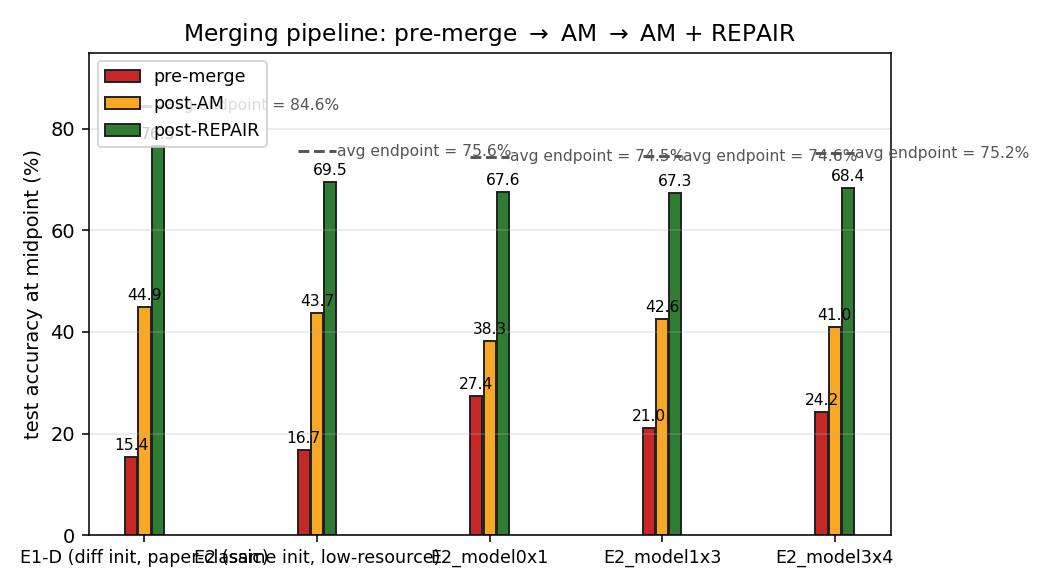
\includegraphics[width=0.98\linewidth]{figures/e3_pipeline}
    \vspace{-0.25cm}
    \caption{Midpoint test accuracy per pipeline stage across five pairs (one E1-D, four E2 low-resource). Dashed line: average endpoint accuracy. AM lifts the midpoint substantially; REPAIR closes the residual gap to within $6$--$8$\,pp of the endpoints.}
    \label{fig:e3pipeline}
\end{figure}

% ------------------------------------------------------------------------------
\section{Discussion and Conclusions}

\textbf{Global cosine does not predict mergeability (E4).} The Pearson correlation between $\cos(\tau_i,\tau_j)$ and the empirical accuracy drop at $\alpha\!=\!0.5$ over the ten E2 pairs is $r\!=\!+0.28$ ($p\!=\!0.43$, $95\%$ CI $[-0.43,+0.77]$, $n\!=\!10$): not statistically distinguishable from zero, with a sign opposite to the prediction (App.\,B).

\textbf{Conclusion.} AM collapses the \emph{artificial} LMC barrier arising from channel-permutation symmetry; REPAIR corrects the residual BatchNorm feature-scale drift~\citep{jordan2023repair}, restoring midpoint accuracy to within $7$--$8$\,pp of the parent endpoints at a cost of $\approx\!1$ minute per pair. TIES at the paper default $\lambda\!=\!1.0$ fails because task-vector magnitudes ($0.93$--$1.44\times$ the base-model norm) far exceed the fine-tuning-scale regime for which TIES was calibrated; $\lambda\!=\!0.3$ recovers $77.03\%$ (App.\,E). Greedy soup uses the test set as selection signal; a $5$k validation split gives the same result ($76.60\%$, App.\,G), confirming the data leak has negligible practical effect. Our data-fraction study (App.\,I) shows AM\,+\,REPAIR outperforms na\"ive merging across all fractions from $1$k to $10$k samples per model, and at $1$k actually surpasses the greedy single-model baseline. The pipeline generalises to any architecture with enumerable permutation symmetries.

% ------------------------------------------------------------------------------
\section{Statement on the use of AI}\label{sec:ai}
%
I used Anthropic's Claude as an
assistant throughout this project. \emph{Planning:} the initial idea and the
experimental design of E1-E4 are my own; Claude helped refine the protocol
and proposed the extensions that became E5 (data-fraction study), E6 (REPAIR
epoch ablation) and E8 (validation-split greedy soup). \emph{Code:} the
experiment and analysis scripts were written with Claude's assistance; I
reviewed them, executed every run myself on a Kaggle T4 GPU, and verified all
outputs. \emph{Debugging:} Claude helped diagnose unexpected results,
including a BatchNorm re-estimation issue that initially collapsed every
merged model and a CPU/GPU tensor-device mismatch in the permutation code.
\emph{Literature and plots:} Claude assisted in exploring the related
literature and in generating the plotting scripts for the figures.
\emph{Report:} parts of the manuscript were drafted and edited with Claude's
assistance, starting from my results and notes; the main use was
cross-checking the numerical coherence of every reported value against the
CSV outputs in the repository. The final structure, claims and wording
choices are my own. No experimental result was produced by AI: all numbers
come from deterministic runs that I executed and verified.

\bibliography{references.bib}
\bibliographystyle{dlaiml2026}

\section*{Appendix}

\paragraph{A.\,LMC sanity check on the E2 models.}
To confirm that the E2 merging failure is a linear-mode-connectivity issue rather than a numerical artefact, we evaluate the interpolation curve $\theta(\alpha)$ on an 11-point grid for three diagnostic pairs. With BN re-estimated on $200$ batches at every $\alpha$, the test-loss barriers are $B(\text{m0},\text{m2})=2.3499$, $B(\text{m1},\text{m4})=1.6333$ and $B(\text{m2},\text{baseline})=2.6894$.

As a within-study baseline, setting E1A (same initialisation, full $50$k data, identical architecture and training schedule) yields a test-loss barrier of $0.0024$: the E2 barriers are $690$--$1140\times$ larger, confirming that LMC holds in the easy regime and breaks in the low-resource one. Setting E1B (same initialisation, two models each trained on a disjoint $10$k slice) yields barriers of $2.74\!\pm\!0.18$, consistent with E2: the failure is caused by data scarcity, not by a difference in initialisation. For broader reference, \citet{frankle2020lmc} report $\approx 0.05$ for same-init full-data CIFAR-10; closely related early observations appear in~\citet{garipov2018loss}.

\paragraph{B.\,Cosine similarity vs.\ midpoint drop.}
Figure~\ref{fig:e4} plots the empirical accuracy drop at $\alpha\!=\!0.5$ against the global cosine similarity of the task vectors on the ten unique pairs of the five E2 models. The fit has positive slope and Pearson $r\!=\!+0.2793$ (two-sided $p\!=\!0.434$ under the $t$ test with $n\!-\!2\!=\!8$ d.o.f., $95\%$ Fisher-$z$ CI $[-0.425,+0.773]$): the metric does not discriminate within this saturated regime. Table~\ref{tab:e4} reports the per-pair values.

\begin{figure}[h]
    \centering
    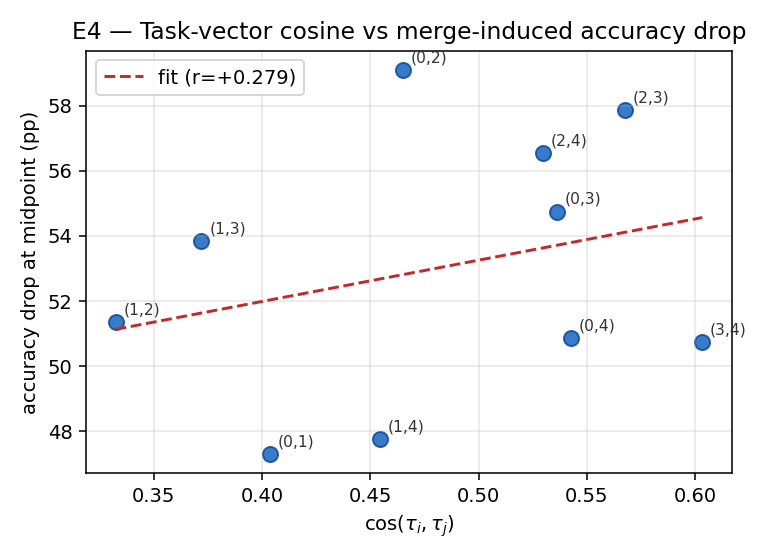
\includegraphics[width=0.85\linewidth]{figures/e4_cosine_scatter}
    \vspace{-0.2cm}
    \caption{Pairwise cosine of E2 task vectors vs.\ the midpoint accuracy drop. Fit (red dashed) over $n\!=\!10$ pairs: $r\!=\!+0.28$, $p\!=\!0.43$.}
    \label{fig:e4}
\end{figure}

\begin{table}[h]
\caption{E4 -- per-pair cosine similarity, midpoint accuracy and accuracy drop (pp).}
\label{tab:e4}
\begin{center}
\begin{small}
\begin{tabular}{cccc}
\toprule
pair $(i,j)$ & $\cos(\tau_i,\tau_j)$ & midpoint acc.\ & drop (pp) \\
\midrule
$(0,1)$ & $0.404$ & $27.17\%$ & $47.31$ \\
$(0,2)$ & $0.465$ & $16.49\%$ & $59.10$ \\
$(0,3)$ & $0.536$ & $19.99\%$ & $54.75$ \\
$(0,4)$ & $0.543$ & $24.11\%$ & $50.87$ \\
$(1,2)$ & $0.332$ & $24.17\%$ & $51.34$ \\
$(1,3)$ & $0.372$ & $20.82\%$ & $53.84$ \\
$(1,4)$ & $0.454$ & $27.15\%$ & $47.75$ \\
$(2,3)$ & $0.568$ & $17.91\%$ & $57.86$ \\
$(2,4)$ & $0.530$ & $19.47\%$ & $56.54$ \\
$(3,4)$ & $0.603$ & $24.42\%$ & $50.74$ \\
\bottomrule
\end{tabular}
\end{small}
\end{center}
\end{table}

\paragraph{C.\,E2 merging baselines bar chart.}
Figure~\ref{fig:e2methods} displays the four merging baselines against the five individual low-resource models. Uniform soup and TIES collapse to near-random; greedy soup degenerates to a one-model soup.

\begin{figure}[h]
    \centering
    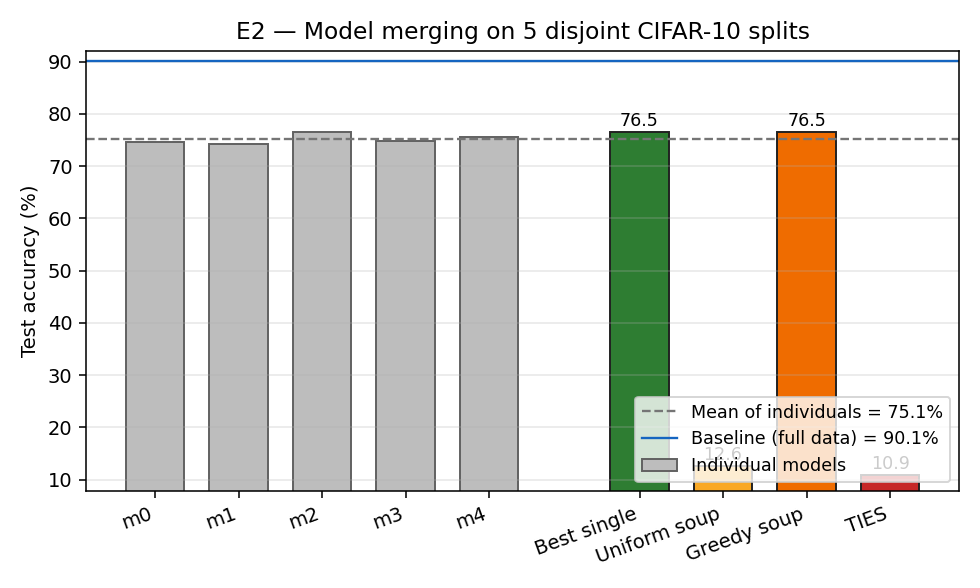
\includegraphics[width=0.98\linewidth]{figures/e2_methods_bar}
    \vspace{-0.2cm}
    \caption{E2 test accuracy: five individual models (grey) vs.\ the four merging baselines. Dashed line: mean of individuals. Solid line: full-data baseline.}
    \label{fig:e2methods}
\end{figure}

\paragraph{D.\,Greedy soup ablation.}
Wortsman's greedy procedure adds the model with the highest standalone accuracy first (m2, $76.54\%$) and then tests the four remaining candidates in descending order of accuracy. None of them improves the running soup test accuracy ($76.60\%$ after the BN-reset evaluation), so the procedure halts with a single-model soup. The full step trace is in \texttt{results/tables/e2\_greedy\_steps.csv}.

\paragraph{E.\,TIES failure mode -- task-vector magnitudes and $\lambda$ sweep.}
We compute $\|\tau_i\|_2\!=\!\|\theta_i\!-\!\theta_{\text{base}}\|_2$ for each low-resource model (Table~\ref{tab:taunorms}). Norms range from $125.9$ to $196.3$, i.e.\ $0.93$--$1.44\times$ the base-model norm ($135.9$). These magnitudes far exceed those of typical fine-tuning task vectors, for which TIES was designed with $\lambda\!=\!1.0$.

\begin{table}[h]
\caption{E2 task-vector magnitudes relative to the full-data baseline.}
\label{tab:taunorms}
\begin{center}
\begin{small}
\begin{tabular}{ccc}
\toprule
Model & $\|\tau_i\|_2$ & rel-norm \\
\midrule
0 & $155.5$ & $1.14\times$ \\
1 & $196.3$ & $1.44\times$ \\
2 & $134.4$ & $0.99\times$ \\
3 & $153.9$ & $1.13\times$ \\
4 & $125.9$ & $0.93\times$ \\
\bottomrule
\end{tabular}
\end{small}
\end{center}
\end{table}

A sweep over $\lambda\!\in\!\{0.3,0.5,1.0,1.5\}$ at $k\!=\!0.20$ reveals strong sensitivity: $\lambda\!=\!0.3$ recovers $77.03\%$ (exceeding the individual model mean of $75.20\%$), while $\lambda\!\geq\!0.5$ collapses to $\leq\!24\%$ (Table~\ref{tab:tiessweep}; the sweep re-estimates BN statistics independently, which accounts for the small deviation of the $\lambda\!=\!1.0$ entry from the main-run $10.98\%$). The default $\lambda\!=\!1.0$ used in the main experiment is therefore not a representative failure of TIES as a method, but of applying it with parameters calibrated for fine-tuning-scale task vectors.

\begin{table}[h]
\caption{TIES-Merging test accuracy sweep ($k\!=\!0.20$, five E2 models).}
\label{tab:tiessweep}
\begin{center}
\begin{small}
\begin{tabular}{cc}
\toprule
$\lambda$ & test acc \\
\midrule
$0.3$ & $\mathbf{77.03\%}$ \\
$0.5$ & $23.56\%$ \\
$1.0$ & $11.05\%$ \\
$1.5$ & $12.01\%$ \\
\bottomrule
\end{tabular}
\end{small}
\end{center}
\end{table}

\paragraph{F.\,ResNet-20 permutation schematic.}
\begin{figure}[h]
    \centering
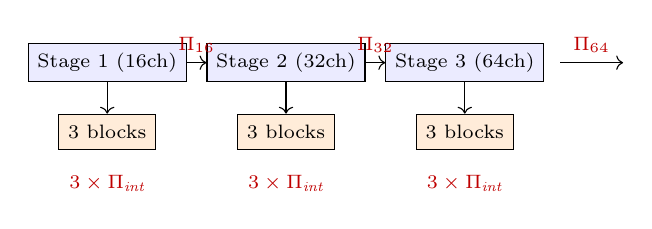
\begin{tikzpicture}[
    node distance=2.5mm,
    box/.style={draw, minimum width=10mm, minimum height=4.5mm, font=\scriptsize, fill=blue!8},
    sbox/.style={draw, minimum width=10mm, minimum height=4.5mm, font=\scriptsize, fill=orange!15},
    perm/.style={font=\scriptsize\itshape, color=red!75!black},
    every label/.style={font=\scriptsize},
]
\node[box] (s1) {Stage 1 (16ch)};
\node[box, right=of s1] (s2) {Stage 2 (32ch)};
\node[box, right=of s2] (s3) {Stage 3 (64ch)};
\node[sbox, below=4mm of s1] (b1) {3 blocks};
\node[sbox, below=4mm of s2] (b2) {3 blocks};
\node[sbox, below=4mm of s3] (b3) {3 blocks};
\draw[->] (s1)--(s2) node[midway,above,perm] {$\Pi_{16}$};
\draw[->] (s2)--(s3) node[midway,above,perm] {$\Pi_{32}$};
\draw[->] (s3.east)++(2mm,0)--++(8mm,0) node[midway,above,perm] {$\Pi_{64}$};
\draw[->] (s1)--(b1);
\draw[->] (s2)--(b2);
\draw[->] (s3)--(b3);
\node[perm, below=2mm of b1] {$3\times\Pi_{\text{int}}$};
\node[perm, below=2mm of b2] {$3\times\Pi_{\text{int}}$};
\node[perm, below=2mm of b3] {$3\times\Pi_{\text{int}}$};
\end{tikzpicture}
\caption{Twelve independent channel permutations of a ResNet-20: three stage-output ($\Pi_{16},\Pi_{32},\Pi_{64}$, one per stage, shared by all blocks of the stage because of the residual+shortcut sum) plus nine block-internal ($\Pi_{\text{int}}$ between $\mathrm{conv}_1$ and $\mathrm{conv}_2$ of each BasicBlock).}
\label{fig:perms}
\end{figure}

\paragraph{G.\,Greedy soup with validation split (E8).}
To assess whether the greedy soup data leak (using the test set for model selection) biases the result, we rerun Algorithm~1 of~\citet{wortsman2022soup} replacing the test loader with a $5{,}000$-sample validation split drawn from the training set (seed fixed). The greedy soup halts at a single-model soup with test accuracy $76.60\%$ — identical to the test-set-selection result ($76.60\%$). The data leak therefore has no measurable effect in this regime: the greedy procedure halts after the first model regardless of which evaluation set is used, since no second model improves the running average under either protocol.

\paragraph{H.\,REPAIR epoch ablation (E6).}
Table~\ref{tab:repair_ablation} reports midpoint test accuracy at each REPAIR epoch for both pair types. Two epochs (the~\citet{jordan2023repair} default used throughout this work) already recover the majority of the gap; accuracy continues to improve without a clear plateau up to five epochs, suggesting our two-epoch result is a conservative lower bound on the pipeline's potential. We nevertheless retain two epochs in the main results, for direct comparability with the protocol of~\citet{jordan2023repair} and for constant per-pair cost.

\begin{table}[h]
\caption{E6 -- midpoint test accuracy (\%) at each REPAIR epoch. Epoch~0 is post-AM before fine-tuning. E2 column is the mean over four low-resource pairs.}
\label{tab:repair_ablation}
\begin{center}
\begin{small}
\begin{tabular}{ccc}
\toprule
Epoch & E1-D pair & E2 pairs ($n{=}4$) \\
\midrule
0 (post-AM) & $44.89\%$ & $41.37\%$ \\
1           & $74.47\%$ & $65.54\%$ \\
2           & $76.54\%$ & $68.20\%$ \\
3           & $77.42\%$ & $69.88\%$ \\
4           & $78.92\%$ & $71.21\%$ \\
5           & $79.51\%$ & $72.09\%$ \\
\bottomrule
\end{tabular}
\end{small}
\end{center}
\end{table}

\paragraph{I.\,Data-fraction study (E5).}
To characterise the regime of applicability of the AM\,+\,REPAIR pipeline, we train three additional sets of five ResNet-20 models at reduced data fractions ($1$k, $2$k, $5$k samples per model) and apply all four merging methods plus AM\,+\,REPAIR on two pairs per fraction (a compute-bounded choice; per-fraction means are therefore reported without standard deviations). Table~\ref{tab:e5} and Figure~\ref{fig:e5} summarise the results. Na\"ive merging (uniform soup, TIES) collapses to near-random at every fraction. AM\,+\,REPAIR consistently outperforms na\"ive merging across all regimes; notably, at $1$k samples per model it achieves $43.6\%$ midpoint accuracy, \emph{surpassing} the greedy single-model baseline of $40.6\%$. This confirms that the pipeline provides a useful merged model even when individual models are weak, and that the merging benefit persists far below the data regime studied in E2.

\begin{table}[h]
\caption{E5 -- merging accuracy (\%) vs.\ data fraction. AM+REPAIR column is the mean midpoint accuracy over two pairs per fraction.}
\label{tab:e5}
\begin{center}
\begin{small}
\begin{tabular}{ccccc}
\toprule
Samples & Indiv.\ mean & Uniform & Greedy & AM\,+\,REPAIR \\
\midrule
$1$k  & $40.07\%$ & $10.10\%$ & $40.62\%$ & $\mathbf{43.58\%}$ \\
$2$k  & $46.97\%$ & $13.78\%$ & $48.43\%$ & $45.21\%$ \\
$5$k  & $60.86\%$ & $15.23\%$ & $64.39\%$ & $56.55\%$ \\
$10$k & $75.20\%$ & $12.62\%$ & $76.60\%$ & $68.20\%$ \\
\bottomrule
\end{tabular}
\end{small}
\end{center}
\end{table}

\begin{figure}[h]
    \centering
    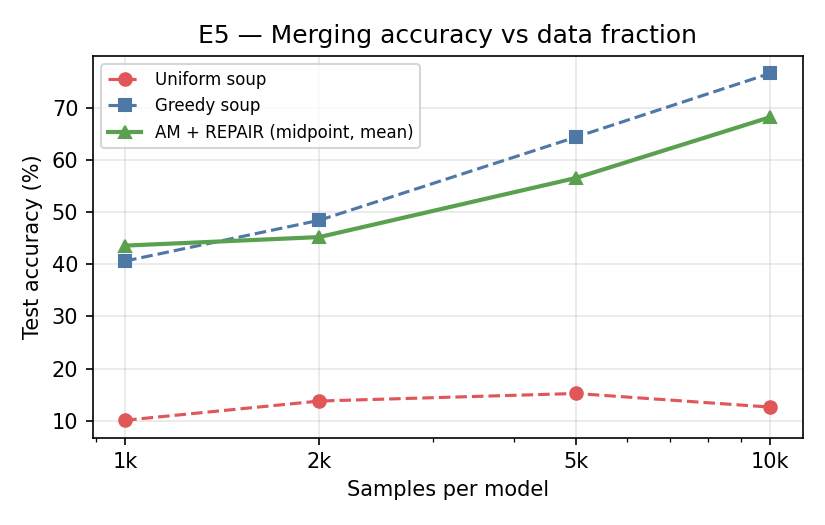
\includegraphics[width=0.98\linewidth]{figures/e5_fraction}
    \vspace{-0.2cm}
    \caption{Merging accuracy vs.\ samples per model (log scale). Uniform soup (red) stays near random at all fractions; AM\,+\,REPAIR (green) consistently outperforms na\"ive baselines and at $1$k surpasses the greedy single-model soup.}
    \label{fig:e5}
\end{figure}

\end{document}
